% TikZ export of an LTSpice schematic — generated by LTSpice to PDF (ASC-Parser).
% Source: 07- Orientation Mirror Bug.asc   Skin: Default
%
% Compile on its own:   pdflatex "07- Orientation Mirror Bug.tex"
% Or drop it into a document:
%     \usepackage{standalone}
%     ...
%     \includestandalone{07- Orientation Mirror Bug}
%
% Lengths are in bp (PDF points), so this matches the PDF export 1:1.
\documentclass[border=0pt]{standalone}
\usepackage[T1]{fontenc}
\usepackage[utf8]{inputenc}
\usepackage{lmodern}
\usepackage{textcomp}
\usepackage{tikz}
\begin{document}
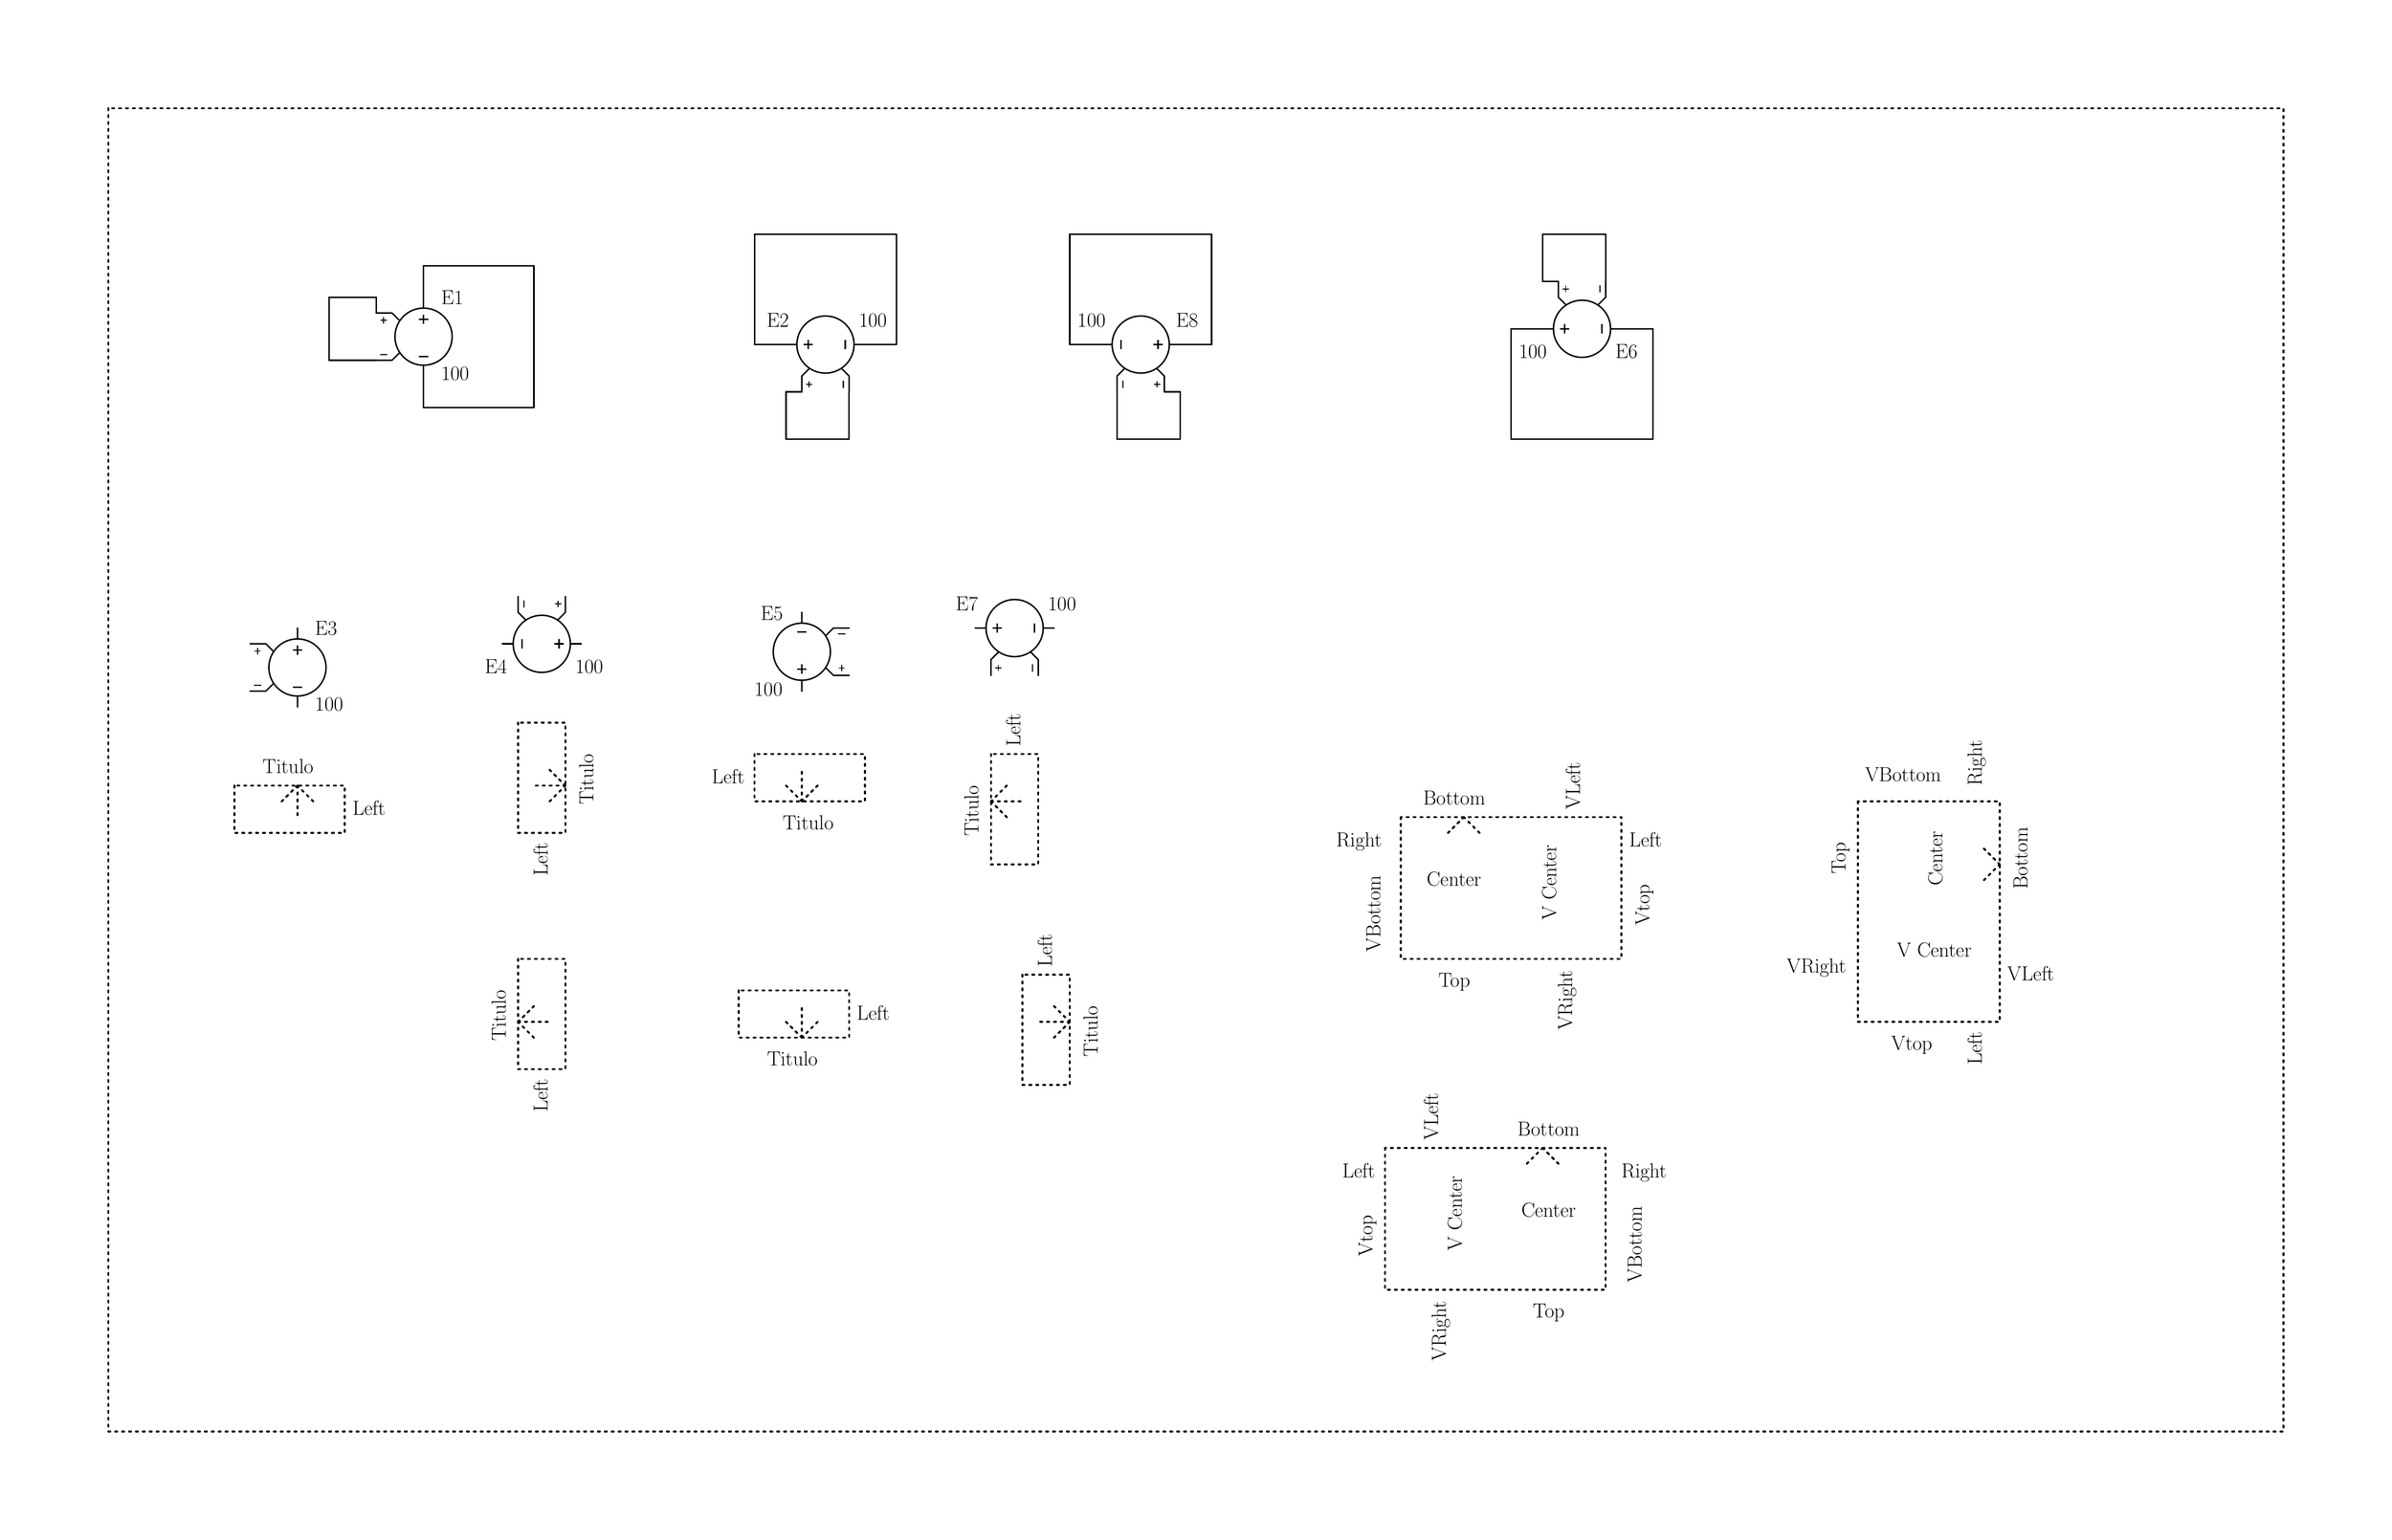
\begin{tikzpicture}[x=1bp, y=1bp, line cap=round, line join=round]
  \useasboundingbox (0,0) rectangle (2408,-1544);
  \path[draw=black, line width=2bp, dash pattern=on 2bp off 5bp] (100,-100) rectangle (2308,-1444);
  \path[draw=black, line width=2bp, dash pattern=on 2bp off 5bp] (228,-788) rectangle (340,-836);
  \path[draw=black, line width=2bp, dash pattern=on 2bp off 5bp] (516,-724) rectangle (564,-836);
  \path[draw=black, line width=2bp, dash pattern=on 2bp off 5bp] (756,-756) rectangle (868,-804);
  \path[draw=black, line width=2bp, dash pattern=on 2bp off 5bp] (996,-756) rectangle (1044,-868);
  \path[draw=black, line width=2bp, dash pattern=on 2bp off 5bp] (516,-964) rectangle (564,-1076);
  \path[draw=black, line width=2bp, dash pattern=on 2bp off 5bp] (740,-996) rectangle (852,-1044);
  \path[draw=black, line width=2bp, dash pattern=on 2bp off 5bp] (1028,-980) rectangle (1076,-1092);
  \path[draw=black, line width=2bp, dash pattern=on 2bp off 5bp] (1412,-820) rectangle (1636,-964);
  \path[draw=black, line width=2bp, dash pattern=on 2bp off 5bp] (1876,-804) rectangle (2020,-1028);
  \path[draw=black, line width=2bp, dash pattern=on 2bp off 5bp] (1396,-1156) rectangle (1620,-1300);
  \path[draw=black, line width=2bp, dash pattern=on 2bp off 5bp] (292,-788) -- (292,-820);
  \path[draw=black, line width=2bp, dash pattern=on 2bp off 5bp] (276,-804) -- (292,-788);
  \path[draw=black, line width=2bp, dash pattern=on 2bp off 5bp] (292,-788) -- (276,-804);
  \path[draw=black, line width=2bp, dash pattern=on 2bp off 5bp] (308,-804) -- (292,-788);
  \path[draw=black, line width=2bp, dash pattern=on 2bp off 5bp] (564,-788) -- (532,-788);
  \path[draw=black, line width=2bp, dash pattern=on 2bp off 5bp] (548,-772) -- (564,-788);
  \path[draw=black, line width=2bp, dash pattern=on 2bp off 5bp] (564,-788) -- (548,-772);
  \path[draw=black, line width=2bp, dash pattern=on 2bp off 5bp] (548,-804) -- (564,-788);
  \path[draw=black, line width=2bp, dash pattern=on 2bp off 5bp] (804,-804) -- (804,-772);
  \path[draw=black, line width=2bp, dash pattern=on 2bp off 5bp] (820,-788) -- (804,-804);
  \path[draw=black, line width=2bp, dash pattern=on 2bp off 5bp] (804,-804) -- (820,-788);
  \path[draw=black, line width=2bp, dash pattern=on 2bp off 5bp] (788,-788) -- (804,-804);
  \path[draw=black, line width=2bp, dash pattern=on 2bp off 5bp] (996,-804) -- (1028,-804);
  \path[draw=black, line width=2bp, dash pattern=on 2bp off 5bp] (1012,-820) -- (996,-804);
  \path[draw=black, line width=2bp, dash pattern=on 2bp off 5bp] (996,-804) -- (1012,-820);
  \path[draw=black, line width=2bp, dash pattern=on 2bp off 5bp] (1012,-788) -- (996,-804);
  \path[draw=black, line width=2bp, dash pattern=on 2bp off 5bp] (516,-1028) -- (548,-1028);
  \path[draw=black, line width=2bp, dash pattern=on 2bp off 5bp] (532,-1012) -- (516,-1028);
  \path[draw=black, line width=2bp, dash pattern=on 2bp off 5bp] (516,-1028) -- (532,-1012);
  \path[draw=black, line width=2bp, dash pattern=on 2bp off 5bp] (532,-1044) -- (516,-1028);
  \path[draw=black, line width=2bp, dash pattern=on 2bp off 5bp] (804,-1044) -- (804,-1012);
  \path[draw=black, line width=2bp, dash pattern=on 2bp off 5bp] (788,-1028) -- (804,-1044);
  \path[draw=black, line width=2bp, dash pattern=on 2bp off 5bp] (804,-1044) -- (788,-1028);
  \path[draw=black, line width=2bp, dash pattern=on 2bp off 5bp] (820,-1028) -- (804,-1044);
  \path[draw=black, line width=2bp, dash pattern=on 2bp off 5bp] (1076,-1028) -- (1044,-1028);
  \path[draw=black, line width=2bp, dash pattern=on 2bp off 5bp] (1060,-1044) -- (1076,-1028);
  \path[draw=black, line width=2bp, dash pattern=on 2bp off 5bp] (1076,-1028) -- (1060,-1044);
  \path[draw=black, line width=2bp, dash pattern=on 2bp off 5bp] (1060,-1012) -- (1076,-1028);
  \path[draw=black, line width=2bp, dash pattern=on 2bp off 5bp] (1460,-836) -- (1476,-820);
  \path[draw=black, line width=2bp, dash pattern=on 2bp off 5bp] (1476,-820) -- (1460,-836);
  \path[draw=black, line width=2bp, dash pattern=on 2bp off 5bp] (1492,-836) -- (1476,-820);
  \path[draw=black, line width=2bp, dash pattern=on 2bp off 5bp] (2004,-852) -- (2020,-868);
  \path[draw=black, line width=2bp, dash pattern=on 2bp off 5bp] (2020,-868) -- (2004,-852);
  \path[draw=black, line width=2bp, dash pattern=on 2bp off 5bp] (2004,-884) -- (2020,-868);
  \path[draw=black, line width=2bp, dash pattern=on 2bp off 5bp] (1572,-1172) -- (1556,-1156);
  \path[draw=black, line width=2bp, dash pattern=on 2bp off 5bp] (1556,-1156) -- (1572,-1172);
  \path[draw=black, line width=2bp, dash pattern=on 2bp off 5bp] (1540,-1172) -- (1556,-1156);
  \path[draw=black, line width=1.5bp] (900,-228) -- (756,-228);
  \path[draw=black, line width=1.5bp] (1220,-228) -- (1076,-228);
  \path[draw=black, line width=1.5bp] (1620,-228) -- (1556,-228);
  \path[draw=black, line width=1.5bp] (532,-260) -- (420,-260);
  \path[draw=black, line width=1.5bp] (1556,-276) -- (1556,-228);
  \path[draw=black, line width=1.5bp] (1572,-276) -- (1556,-276);
  \path[draw=black, line width=1.5bp] (1620,-276) -- (1620,-228);
  \path[draw=black, line width=1.5bp] (372,-292) -- (324,-292);
  \path[draw=black, line width=1.5bp] (420,-292) -- (420,-260);
  \path[draw=black, line width=1.5bp] (372,-308) -- (372,-292);
  \path[draw=black, line width=1.5bp] (1556,-324) -- (1524,-324);
  \path[draw=black, line width=1.5bp] (1668,-324) -- (1636,-324);
  \path[draw=black, line width=1.5bp] (756,-340) -- (756,-228);
  \path[draw=black, line width=1.5bp] (788,-340) -- (756,-340);
  \path[draw=black, line width=1.5bp] (900,-340) -- (900,-228);
  \path[draw=black, line width=1.5bp] (900,-340) -- (868,-340);
  \path[draw=black, line width=1.5bp] (1076,-340) -- (1076,-228);
  \path[draw=black, line width=1.5bp] (1108,-340) -- (1076,-340);
  \path[draw=black, line width=1.5bp] (1220,-340) -- (1220,-228);
  \path[draw=black, line width=1.5bp] (1220,-340) -- (1188,-340);
  \path[draw=black, line width=1.5bp] (324,-356) -- (324,-292);
  \path[draw=black, line width=1.5bp] (372,-356) -- (324,-356);
  \path[draw=black, line width=1.5bp] (804,-388) -- (788,-388);
  \path[draw=black, line width=1.5bp] (1188,-388) -- (1172,-388);
  \path[draw=black, line width=1.5bp] (420,-404) -- (420,-372);
  \path[draw=black, line width=1.5bp] (532,-404) -- (532,-260);
  \path[draw=black, line width=1.5bp] (532,-404) -- (420,-404);
  \path[draw=black, line width=1.5bp] (788,-436) -- (788,-388);
  \path[draw=black, line width=1.5bp] (852,-436) -- (852,-388);
  \path[draw=black, line width=1.5bp] (852,-436) -- (788,-436);
  \path[draw=black, line width=1.5bp] (1124,-436) -- (1124,-388);
  \path[draw=black, line width=1.5bp] (1188,-436) -- (1188,-388);
  \path[draw=black, line width=1.5bp] (1188,-436) -- (1124,-436);
  \path[draw=black, line width=1.5bp] (1524,-436) -- (1524,-324);
  \path[draw=black, line width=1.5bp] (1668,-436) -- (1668,-324);
  \path[draw=black, line width=1.5bp] (1668,-436) -- (1524,-436);
  \path[draw=black, line width=1.5bp] (1556,-324) -- (1567,-324);
  \path[draw=black, line width=1.5bp] (1625,-324) -- (1636,-324);
  \path[draw=black, line width=1.5bp] (1596,-324) ellipse[x radius=29bp, y radius=29bp];
  \path[draw=black, line width=0.5bp] (1616.1,-328) -- (1616.1,-320);
  \path[draw=black, line width=0.5bp, fill=black] (1615.6,-319.5) -- (1615.6,-328.5) -- (1616.6,-328.5) -- (1616.6,-319.5) -- (1615.6,-319.5);
  \path[draw=black, line width=0.39bp] (1614.1,-286.6) -- (1614.1,-280.3);
  \path[draw=black, line width=0.39bp, fill=black] (1613.7,-280) -- (1613.7,-287) -- (1614.5,-287) -- (1614.5,-280) -- (1613.7,-280);
  \path[draw=black, line width=0.5bp, fill=black] (1577.9,-328.5) -- (1577.9,-324.5) -- (1573.9,-324.5) -- (1573.9,-323.5) -- (1577.9,-323.5) -- (1577.9,-319.5) -- (1578.9,-319.5) -- (1578.9,-323.5) -- (1582.9,-323.5) -- (1582.9,-324.5) -- (1578.9,-324.5) -- (1578.9,-328.5) -- (1577.9,-328.5) -- (1577.9,-328.5);
  \path[draw=black, line width=0.33bp, fill=black] (1579.1,-286.5) -- (1579.1,-283.8) -- (1576.4,-283.8) -- (1576.4,-283.1) -- (1579.1,-283.1) -- (1579.1,-280.5) -- (1579.7,-280.5) -- (1579.7,-283.1) -- (1582.4,-283.1) -- (1582.4,-283.8) -- (1579.7,-283.8) -- (1579.7,-286.5) -- (1579.1,-286.5) -- (1579.1,-286.5);
  \path[draw=black, line width=1.5bp] (1579.9,-299.9) -- (1572,-292) -- (1572,-276);
  \path[draw=black, line width=1.5bp] (1620,-276) -- (1620,-292) -- (1612.1,-299.9);
  \node[anchor=base west, inner sep=0pt, outer sep=0pt, font=\fontsize{20bp}{24bp}\selectfont] at (1630,-354) {E6};
  \node[anchor=base west, inner sep=0pt, outer sep=0pt, font=\fontsize{20bp}{24bp}\selectfont] at (1532,-354) {100};
  \path[draw=black, line width=1.5bp] (1188,-340) -- (1177,-340);
  \path[draw=black, line width=1.5bp] (1119,-340) -- (1108,-340);
  \path[draw=black, line width=1.5bp] (1148,-340) ellipse[x radius=29bp, y radius=29bp];
  \path[draw=black, line width=0.5bp] (1127.9,-336) -- (1127.9,-344);
  \path[draw=black, line width=0.5bp, fill=black] (1128.4,-344.5) -- (1128.4,-335.5) -- (1127.4,-335.5) -- (1127.4,-344.5) -- (1128.4,-344.5);
  \path[draw=black, line width=0.39bp] (1129.9,-377.4) -- (1129.9,-383.7);
  \path[draw=black, line width=0.39bp, fill=black] (1130.3,-384) -- (1130.3,-377) -- (1129.5,-377) -- (1129.5,-384) -- (1130.3,-384);
  \path[draw=black, line width=0.5bp, fill=black] (1166.1,-335.5) -- (1166.1,-339.5) -- (1170.1,-339.5) -- (1170.1,-340.5) -- (1166.1,-340.5) -- (1166.1,-344.5) -- (1165.1,-344.5) -- (1165.1,-340.5) -- (1161.1,-340.5) -- (1161.1,-339.5) -- (1165.1,-339.5) -- (1165.1,-335.5) -- (1166.1,-335.5) -- (1166.1,-335.5);
  \path[draw=black, line width=0.33bp, fill=black] (1164.9,-377.5) -- (1164.9,-380.2) -- (1167.6,-380.2) -- (1167.6,-380.9) -- (1164.9,-380.9) -- (1164.9,-383.5) -- (1164.3,-383.5) -- (1164.3,-380.9) -- (1161.6,-380.9) -- (1161.6,-380.2) -- (1164.3,-380.2) -- (1164.3,-377.5) -- (1164.9,-377.5) -- (1164.9,-377.5);
  \path[draw=black, line width=1.5bp] (1164.1,-364.1) -- (1172,-372) -- (1172,-388);
  \path[draw=black, line width=1.5bp] (1124,-388) -- (1124,-372) -- (1131.9,-364.1);
  \node[anchor=base west, inner sep=0pt, outer sep=0pt, font=\fontsize{20bp}{24bp}\selectfont] at (1184,-322) {E8};
  \node[anchor=base west, inner sep=0pt, outer sep=0pt, font=\fontsize{20bp}{24bp}\selectfont] at (1084,-322) {100};
  \path[draw=black, line width=1.5bp] (420,-292) -- (420,-303);
  \path[draw=black, line width=1.5bp] (420,-361) -- (420,-372);
  \path[draw=black, line width=1.5bp] (420,-332) ellipse[x radius=29bp, y radius=29bp];
  \path[draw=black, line width=0.5bp] (424,-352.1) -- (416,-352.1);
  \path[draw=black, line width=0.5bp, fill=black] (415.5,-351.6) -- (424.5,-351.6) -- (424.5,-352.6) -- (415.5,-352.6) -- (415.5,-351.6);
  \path[draw=black, line width=0.39bp] (382.6,-350.1) -- (376.3,-350.1);
  \path[draw=black, line width=0.39bp, fill=black] (376,-349.7) -- (383,-349.7) -- (383,-350.5) -- (376,-350.5) -- (376,-349.7);
  \path[draw=black, line width=0.5bp, fill=black] (424.5,-313.9) -- (420.5,-313.9) -- (420.5,-309.9) -- (419.5,-309.9) -- (419.5,-313.9) -- (415.5,-313.9) -- (415.5,-314.9) -- (419.5,-314.9) -- (419.5,-318.9) -- (420.5,-318.9) -- (420.5,-314.9) -- (424.5,-314.9) -- (424.5,-313.9) -- (424.5,-313.9);
  \path[draw=black, line width=0.33bp, fill=black] (382.5,-315.1) -- (379.8,-315.1) -- (379.8,-312.4) -- (379.1,-312.4) -- (379.1,-315.1) -- (376.5,-315.1) -- (376.5,-315.7) -- (379.1,-315.7) -- (379.1,-318.4) -- (379.8,-318.4) -- (379.8,-315.7) -- (382.5,-315.7) -- (382.5,-315.1) -- (382.5,-315.1);
  \path[draw=black, line width=1.5bp] (395.9,-315.9) -- (388,-308) -- (372,-308);
  \path[draw=black, line width=1.5bp] (372,-356) -- (388,-356) -- (395.9,-348.1);
  \node[anchor=base west, inner sep=0pt, outer sep=0pt, font=\fontsize{20bp}{24bp}\selectfont] at (438,-299) {E1};
  \node[anchor=base west, inner sep=0pt, outer sep=0pt, font=\fontsize{20bp}{24bp}\selectfont] at (438,-376) {100};
  \path[draw=black, line width=1.5bp] (788,-340) -- (799,-340);
  \path[draw=black, line width=1.5bp] (857,-340) -- (868,-340);
  \path[draw=black, line width=1.5bp] (828,-340) ellipse[x radius=29bp, y radius=29bp];
  \path[draw=black, line width=0.5bp] (848.1,-336) -- (848.1,-344);
  \path[draw=black, line width=0.5bp, fill=black] (847.6,-344.5) -- (847.6,-335.5) -- (848.6,-335.5) -- (848.6,-344.5) -- (847.6,-344.5);
  \path[draw=black, line width=0.39bp] (846.1,-377.4) -- (846.1,-383.7);
  \path[draw=black, line width=0.39bp, fill=black] (845.7,-384) -- (845.7,-377) -- (846.5,-377) -- (846.5,-384) -- (845.7,-384);
  \path[draw=black, line width=0.5bp, fill=black] (809.9,-335.5) -- (809.9,-339.5) -- (805.9,-339.5) -- (805.9,-340.5) -- (809.9,-340.5) -- (809.9,-344.5) -- (810.9,-344.5) -- (810.9,-340.5) -- (814.9,-340.5) -- (814.9,-339.5) -- (810.9,-339.5) -- (810.9,-335.5) -- (809.9,-335.5) -- (809.9,-335.5);
  \path[draw=black, line width=0.33bp, fill=black] (811.1,-377.5) -- (811.1,-380.2) -- (808.4,-380.2) -- (808.4,-380.9) -- (811.1,-380.9) -- (811.1,-383.5) -- (811.7,-383.5) -- (811.7,-380.9) -- (814.4,-380.9) -- (814.4,-380.2) -- (811.7,-380.2) -- (811.7,-377.5) -- (811.1,-377.5) -- (811.1,-377.5);
  \path[draw=black, line width=1.5bp] (811.9,-364.1) -- (804,-372) -- (804,-388);
  \path[draw=black, line width=1.5bp] (852,-388) -- (852,-372) -- (844.1,-364.1);
  \node[anchor=base west, inner sep=0pt, outer sep=0pt, font=\fontsize{20bp}{24bp}\selectfont] at (768.38,-322) {E2};
  \node[anchor=base west, inner sep=0pt, outer sep=0pt, font=\fontsize{20bp}{24bp}\selectfont] at (862,-322) {100};
  \path[draw=black, line width=1.5bp] (292,-628) -- (292,-639);
  \path[draw=black, line width=1.5bp] (292,-697) -- (292,-708);
  \path[draw=black, line width=1.5bp] (292,-668) ellipse[x radius=29bp, y radius=29bp];
  \path[draw=black, line width=0.5bp] (296,-688.1) -- (288,-688.1);
  \path[draw=black, line width=0.5bp, fill=black] (287.5,-687.6) -- (296.5,-687.6) -- (296.5,-688.6) -- (287.5,-688.6) -- (287.5,-687.6);
  \path[draw=black, line width=0.39bp] (254.6,-686.1) -- (248.3,-686.1);
  \path[draw=black, line width=0.39bp, fill=black] (248,-685.7) -- (255,-685.7) -- (255,-686.5) -- (248,-686.5) -- (248,-685.7);
  \path[draw=black, line width=0.5bp, fill=black] (296.5,-649.9) -- (292.5,-649.9) -- (292.5,-645.9) -- (291.5,-645.9) -- (291.5,-649.9) -- (287.5,-649.9) -- (287.5,-650.9) -- (291.5,-650.9) -- (291.5,-654.9) -- (292.5,-654.9) -- (292.5,-650.9) -- (296.5,-650.9) -- (296.5,-649.9) -- (296.5,-649.9);
  \path[draw=black, line width=0.33bp, fill=black] (254.5,-651.1) -- (251.8,-651.1) -- (251.8,-648.4) -- (251.1,-648.4) -- (251.1,-651.1) -- (248.5,-651.1) -- (248.5,-651.7) -- (251.1,-651.7) -- (251.1,-654.4) -- (251.8,-654.4) -- (251.8,-651.7) -- (254.5,-651.7) -- (254.5,-651.1) -- (254.5,-651.1);
  \path[draw=black, line width=1.5bp] (267.9,-651.9) -- (260,-644) -- (244,-644);
  \path[draw=black, line width=1.5bp] (244,-692) -- (260,-692) -- (267.9,-684.1);
  \node[anchor=base west, inner sep=0pt, outer sep=0pt, font=\fontsize{20bp}{24bp}\selectfont] at (310,-635) {E3};
  \node[anchor=base west, inner sep=0pt, outer sep=0pt, font=\fontsize{20bp}{24bp}\selectfont] at (310,-712) {100};
  \path[draw=black, line width=1.5bp] (580,-644) -- (569,-644);
  \path[draw=black, line width=1.5bp] (511,-644) -- (500,-644);
  \path[draw=black, line width=1.5bp] (540,-644) ellipse[x radius=29bp, y radius=29bp];
  \path[draw=black, line width=0.5bp] (519.9,-648) -- (519.9,-640);
  \path[draw=black, line width=0.5bp, fill=black] (520.4,-639.5) -- (520.4,-648.5) -- (519.4,-648.5) -- (519.4,-639.5) -- (520.4,-639.5);
  \path[draw=black, line width=0.39bp] (521.9,-606.6) -- (521.9,-600.3);
  \path[draw=black, line width=0.39bp, fill=black] (522.3,-600) -- (522.3,-607) -- (521.5,-607) -- (521.5,-600) -- (522.3,-600);
  \path[draw=black, line width=0.5bp, fill=black] (558.1,-648.5) -- (558.1,-644.5) -- (562.1,-644.5) -- (562.1,-643.5) -- (558.1,-643.5) -- (558.1,-639.5) -- (557.1,-639.5) -- (557.1,-643.5) -- (553.1,-643.5) -- (553.1,-644.5) -- (557.1,-644.5) -- (557.1,-648.5) -- (558.1,-648.5) -- (558.1,-648.5);
  \path[draw=black, line width=0.33bp, fill=black] (556.9,-606.5) -- (556.9,-603.8) -- (559.6,-603.8) -- (559.6,-603.1) -- (556.9,-603.1) -- (556.9,-600.5) -- (556.3,-600.5) -- (556.3,-603.1) -- (553.6,-603.1) -- (553.6,-603.8) -- (556.3,-603.8) -- (556.3,-606.5) -- (556.9,-606.5) -- (556.9,-606.5);
  \path[draw=black, line width=1.5bp] (556.1,-619.9) -- (564,-612) -- (564,-596);
  \path[draw=black, line width=1.5bp] (516,-596) -- (516,-612) -- (523.9,-619.9);
  \node[anchor=base west, inner sep=0pt, outer sep=0pt, font=\fontsize{20bp}{24bp}\selectfont] at (482.38,-674) {E4};
  \node[anchor=base west, inner sep=0pt, outer sep=0pt, font=\fontsize{20bp}{24bp}\selectfont] at (574,-674) {100};
  \path[draw=black, line width=1.5bp] (804,-692) -- (804,-681);
  \path[draw=black, line width=1.5bp] (804,-623) -- (804,-612);
  \path[draw=black, line width=1.5bp] (804,-652) ellipse[x radius=29bp, y radius=29bp];
  \path[draw=black, line width=0.5bp] (800,-631.9) -- (808,-631.9);
  \path[draw=black, line width=0.5bp, fill=black] (808.5,-632.4) -- (799.5,-632.4) -- (799.5,-631.4) -- (808.5,-631.4) -- (808.5,-632.4);
  \path[draw=black, line width=0.39bp] (841.4,-633.9) -- (847.7,-633.9);
  \path[draw=black, line width=0.39bp, fill=black] (848,-634.3) -- (841,-634.3) -- (841,-633.5) -- (848,-633.5) -- (848,-634.3);
  \path[draw=black, line width=0.5bp, fill=black] (799.5,-670.1) -- (803.5,-670.1) -- (803.5,-674.1) -- (804.5,-674.1) -- (804.5,-670.1) -- (808.5,-670.1) -- (808.5,-669.1) -- (804.5,-669.1) -- (804.5,-665.1) -- (803.5,-665.1) -- (803.5,-669.1) -- (799.5,-669.1) -- (799.5,-670.1) -- (799.5,-670.1);
  \path[draw=black, line width=0.33bp, fill=black] (841.5,-668.9) -- (844.2,-668.9) -- (844.2,-671.6) -- (844.9,-671.6) -- (844.9,-668.9) -- (847.5,-668.9) -- (847.5,-668.3) -- (844.9,-668.3) -- (844.9,-665.6) -- (844.2,-665.6) -- (844.2,-668.3) -- (841.5,-668.3) -- (841.5,-668.9) -- (841.5,-668.9);
  \path[draw=black, line width=1.5bp] (828.1,-668.1) -- (836,-676) -- (852,-676);
  \path[draw=black, line width=1.5bp] (852,-628) -- (836,-628) -- (828.1,-635.9);
  \node[anchor=base west, inner sep=0pt, outer sep=0pt, font=\fontsize{20bp}{24bp}\selectfont] at (762.38,-620) {E5};
  \node[anchor=base west, inner sep=0pt, outer sep=0pt, font=\fontsize{20bp}{24bp}\selectfont] at (756,-697) {100};
  \path[draw=black, line width=1.5bp] (980,-628) -- (991,-628);
  \path[draw=black, line width=1.5bp] (1049,-628) -- (1060,-628);
  \path[draw=black, line width=1.5bp] (1020,-628) ellipse[x radius=29bp, y radius=29bp];
  \path[draw=black, line width=0.5bp] (1040.1,-624) -- (1040.1,-632);
  \path[draw=black, line width=0.5bp, fill=black] (1039.6,-632.5) -- (1039.6,-623.5) -- (1040.6,-623.5) -- (1040.6,-632.5) -- (1039.6,-632.5);
  \path[draw=black, line width=0.39bp] (1038.1,-665.4) -- (1038.1,-671.7);
  \path[draw=black, line width=0.39bp, fill=black] (1037.7,-672) -- (1037.7,-665) -- (1038.5,-665) -- (1038.5,-672) -- (1037.7,-672);
  \path[draw=black, line width=0.5bp, fill=black] (1001.9,-623.5) -- (1001.9,-627.5) -- (997.9,-627.5) -- (997.9,-628.5) -- (1001.9,-628.5) -- (1001.9,-632.5) -- (1002.9,-632.5) -- (1002.9,-628.5) -- (1006.9,-628.5) -- (1006.9,-627.5) -- (1002.9,-627.5) -- (1002.9,-623.5) -- (1001.9,-623.5) -- (1001.9,-623.5);
  \path[draw=black, line width=0.33bp, fill=black] (1003.1,-665.5) -- (1003.1,-668.2) -- (1000.4,-668.2) -- (1000.4,-668.9) -- (1003.1,-668.9) -- (1003.1,-671.5) -- (1003.7,-671.5) -- (1003.7,-668.9) -- (1006.4,-668.9) -- (1006.4,-668.2) -- (1003.7,-668.2) -- (1003.7,-665.5) -- (1003.1,-665.5) -- (1003.1,-665.5);
  \path[draw=black, line width=1.5bp] (1003.9,-652.1) -- (996,-660) -- (996,-676);
  \path[draw=black, line width=1.5bp] (1044,-676) -- (1044,-660) -- (1036.1,-652.1);
  \node[anchor=base west, inner sep=0pt, outer sep=0pt, font=\fontsize{20bp}{24bp}\selectfont] at (960.38,-610) {E7};
  \node[anchor=base west, inner sep=0pt, outer sep=0pt, font=\fontsize{20bp}{24bp}\selectfont] at (1054,-610) {100};
  \node[anchor=base west, inner sep=0pt, outer sep=0pt, font=\fontsize{20bp}{24bp}\selectfont] at (256.77,-775.5) {Titulo};
  \node[anchor=base west, inner sep=0pt, outer sep=0pt, font=\fontsize{20bp}{24bp}\selectfont] at (348,-818) {Left};
  \node[anchor=base west, inner sep=0pt, outer sep=0pt, rotate=90, font=\fontsize{20bp}{24bp}\selectfont] at (592.5,-807.23) {Titulo};
  \node[anchor=base west, inner sep=0pt, outer sep=0pt, rotate=90, font=\fontsize{20bp}{24bp}\selectfont] at (546,-879.28) {Left};
  \node[anchor=base west, inner sep=0pt, outer sep=0pt, font=\fontsize{20bp}{24bp}\selectfont] at (784.77,-832.5) {Titulo};
  \node[anchor=base west, inner sep=0pt, outer sep=0pt, font=\fontsize{20bp}{24bp}\selectfont] at (712.72,-786) {Left};
  \node[anchor=base west, inner sep=0pt, outer sep=0pt, rotate=90, font=\fontsize{20bp}{24bp}\selectfont] at (983.5,-839.23) {Titulo};
  \node[anchor=base west, inner sep=0pt, outer sep=0pt, rotate=90, font=\fontsize{20bp}{24bp}\selectfont] at (1026,-748) {Left};
  \node[anchor=base west, inner sep=0pt, outer sep=0pt, rotate=90, font=\fontsize{20bp}{24bp}\selectfont] at (503.5,-1047.23) {Titulo};
  \node[anchor=base west, inner sep=0pt, outer sep=0pt, rotate=90, font=\fontsize{20bp}{24bp}\selectfont] at (546,-1119.28) {Left};
  \node[anchor=base west, inner sep=0pt, outer sep=0pt, font=\fontsize{20bp}{24bp}\selectfont] at (768.77,-1072.5) {Titulo};
  \node[anchor=base west, inner sep=0pt, outer sep=0pt, font=\fontsize{20bp}{24bp}\selectfont] at (860,-1026) {Left};
  \node[anchor=base west, inner sep=0pt, outer sep=0pt, rotate=90, font=\fontsize{20bp}{24bp}\selectfont] at (1104.5,-1063.23) {Titulo};
  \node[anchor=base west, inner sep=0pt, outer sep=0pt, rotate=90, font=\fontsize{20bp}{24bp}\selectfont] at (1058,-972) {Left};
  \node[anchor=base west, inner sep=0pt, outer sep=0pt, font=\fontsize{20bp}{24bp}\selectfont] at (1434.81,-807.5) {Bottom};
  \node[anchor=base west, inner sep=0pt, outer sep=0pt, font=\fontsize{20bp}{24bp}\selectfont] at (1644,-850) {Left};
  \node[anchor=base west, inner sep=0pt, outer sep=0pt, font=\fontsize{20bp}{24bp}\selectfont] at (1346.82,-850) {Right};
  \node[anchor=base west, inner sep=0pt, outer sep=0pt, font=\fontsize{20bp}{24bp}\selectfont] at (1450.22,-992.5) {Top};
  \node[anchor=base west, inner sep=0pt, outer sep=0pt, rotate=90, font=\fontsize{20bp}{24bp}\selectfont] at (1570,-924.3) {V Center};
  \node[anchor=base west, inner sep=0pt, outer sep=0pt, rotate=90, font=\fontsize{20bp}{24bp}\selectfont] at (1391.5,-956.69) {VBottom};
  \node[anchor=base west, inner sep=0pt, outer sep=0pt, rotate=90, font=\fontsize{20bp}{24bp}\selectfont] at (1664.5,-929.95) {Vtop};
  \node[anchor=base west, inner sep=0pt, outer sep=0pt, rotate=90, font=\fontsize{20bp}{24bp}\selectfont] at (1594,-812) {VLeft};
  \node[anchor=base west, inner sep=0pt, outer sep=0pt, rotate=90, font=\fontsize{20bp}{24bp}\selectfont] at (1586,-1036.18) {VRight};
  \node[anchor=base west, inner sep=0pt, outer sep=0pt, font=\fontsize{20bp}{24bp}\selectfont] at (1438.53,-890) {Center};
  \node[anchor=base west, inner sep=0pt, outer sep=0pt, rotate=90, font=\fontsize{20bp}{24bp}\selectfont] at (2048.5,-893.19) {Bottom};
  \node[anchor=base west, inner sep=0pt, outer sep=0pt, rotate=90, font=\fontsize{20bp}{24bp}\selectfont] at (2002,-1071.28) {Left};
  \node[anchor=base west, inner sep=0pt, outer sep=0pt, rotate=90, font=\fontsize{20bp}{24bp}\selectfont] at (2002,-788) {Right};
  \node[anchor=base west, inner sep=0pt, outer sep=0pt, rotate=90, font=\fontsize{20bp}{24bp}\selectfont] at (1863.5,-877.78) {Top};
  \node[anchor=base west, inner sep=0pt, outer sep=0pt, font=\fontsize{20bp}{24bp}\selectfont] at (1915.7,-962) {V Center};
  \node[anchor=base west, inner sep=0pt, outer sep=0pt, font=\fontsize{20bp}{24bp}\selectfont] at (1883.31,-783.5) {VBottom};
  \node[anchor=base west, inner sep=0pt, outer sep=0pt, font=\fontsize{20bp}{24bp}\selectfont] at (1910.05,-1056.5) {Vtop};
  \node[anchor=base west, inner sep=0pt, outer sep=0pt, font=\fontsize{20bp}{24bp}\selectfont] at (2028,-986) {VLeft};
  \node[anchor=base west, inner sep=0pt, outer sep=0pt, font=\fontsize{20bp}{24bp}\selectfont] at (1803.82,-978) {VRight};
  \node[anchor=base west, inner sep=0pt, outer sep=0pt, rotate=90, font=\fontsize{20bp}{24bp}\selectfont] at (1962,-889.47) {Center};
  \node[anchor=base west, inner sep=0pt, outer sep=0pt, font=\fontsize{20bp}{24bp}\selectfont] at (1530.81,-1143.5) {Bottom};
  \node[anchor=base west, inner sep=0pt, outer sep=0pt, font=\fontsize{20bp}{24bp}\selectfont] at (1352.72,-1186) {Left};
  \node[anchor=base west, inner sep=0pt, outer sep=0pt, font=\fontsize{20bp}{24bp}\selectfont] at (1636,-1186) {Right};
  \node[anchor=base west, inner sep=0pt, outer sep=0pt, font=\fontsize{20bp}{24bp}\selectfont] at (1546.22,-1328.5) {Top};
  \node[anchor=base west, inner sep=0pt, outer sep=0pt, rotate=90, font=\fontsize{20bp}{24bp}\selectfont] at (1474,-1260.3) {V Center};
  \node[anchor=base west, inner sep=0pt, outer sep=0pt, rotate=90, font=\fontsize{20bp}{24bp}\selectfont] at (1656.5,-1292.69) {VBottom};
  \node[anchor=base west, inner sep=0pt, outer sep=0pt, rotate=90, font=\fontsize{20bp}{24bp}\selectfont] at (1383.5,-1265.95) {Vtop};
  \node[anchor=base west, inner sep=0pt, outer sep=0pt, rotate=90, font=\fontsize{20bp}{24bp}\selectfont] at (1450,-1148) {VLeft};
  \node[anchor=base west, inner sep=0pt, outer sep=0pt, rotate=90, font=\fontsize{20bp}{24bp}\selectfont] at (1458,-1372.18) {VRight};
  \node[anchor=base west, inner sep=0pt, outer sep=0pt, font=\fontsize{20bp}{24bp}\selectfont] at (1534.53,-1226) {Center};
\end{tikzpicture}
\end{document}
